\documentclass[a4paper,12pt]{article}
\usepackage{dingbat}
\usepackage{pifont}
\usepackage{hyperref}
\usepackage{graphicx}
\usepackage{listings}
\graphicspath{{images/}}

\begin{document}
\newcommand{\xmark}{\ding{55}}

\author{Wannes Fransen}
\title{3D Bin Packing - Program Technical Report}

\section{Technical report: Packing program}
This document is meant to specify what exactly happens in the current program. Here we can see what the opportunities, limitations, upsides and downsides are. Often will details be explained with either code blocks or class diagrams. 

\subsection{Minimal requirements}
Every program has the minimum amount of features to function properly. Making a program decently requires a lot of time, extensive testing and a lot of communication with the client and other developers. \\ 

Therefore, I'll be honest and say that the program is, in my opinion, not yet completely finished and ready to be used in a commercial environment due to mostly lack of time and experience. Though it is ready to be used as a reference for proving theoretical problems, packing columns in boxes (with possible human intervention), etc... \\

\paragraph{Must-have features}
\begin{itemize}
	\item[] \checkmark Algorithmic approach: Pack columns in boxes.
	\item[] \checkmark Algorithmic approach: Calculate best combination
	\item[] \checkmark Compatibility: other front-ends
	\item[] \checkmark Basic visualization
	\item[] \xmark \space Extensive testing
	\item[] \xmark \space Error handling \\
\end{itemize}

\paragraph{Optional features}
\begin{itemize}
	\item Web based configuration: boxes management (update sizes, etc...)
	\item Integrate cost regression and link the projects
	\item visualization: short \& detailed calculation (no layer schematics)
	\item dependency injection
\end{itemize}

\paragraph{Todo list:} 
There are still some small changes to be made. The newest version is updated on our \hyperref{https://github.com/WannesFransen1994/3D_Bin_Packaging}{}{}{git repository}*.\\
\small \textit{Please do keep in mind that different students worked at this project. Not every commit is as it should be, or is professionally written.}
\begin{itemize}
	\item[] \checkmark Update class names (Box = Column, Container = Box)
	\item[] \checkmark Review constructors usage
	\item[] \checkmark No calculations in Facade
	\item[] \checkmark Correctly implement Strategy pattern
	\item[] \xmark \space Copy constructor sort keys based on coordinates
\end{itemize}
\pagebreak

\subsection{Class diagram: General overview}
Here is a short overview. This diagram is generated through IntelliJ IDEA.\\

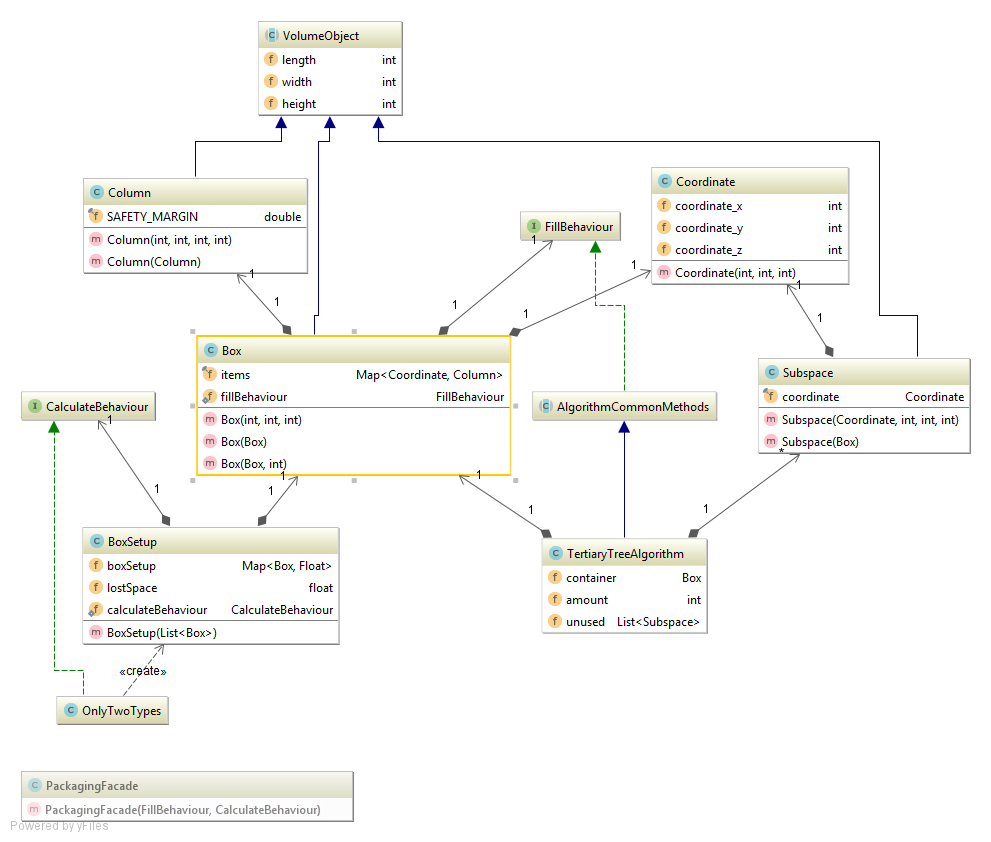
\includegraphics[width=17cm]{Class_diagram_overview2.png}\\

There are 3 parts in this program with their respective classes. There are more classes, but those are referenced in either a general context (Factory classes) or are entities (Column, Coordinate, Subspace, etc...). 
\begin{enumerate}
	\item The Facade: which is responsible for all communication with other programs. The rest service will communicate entirely through this class, but the class is not allowed to have any logic behind it.
	\item The packing algorithm classes: Box (and the static methods), FillBehaviour, TertiaryTreeAlgorithm.
	\item The optimal setup algorithm classes: OnlyTwoTypes, BoxSetup, CalculateBehaviour.
\end{enumerate}

\pagebreak

\subsection{Class diagram: Packing algorithm}
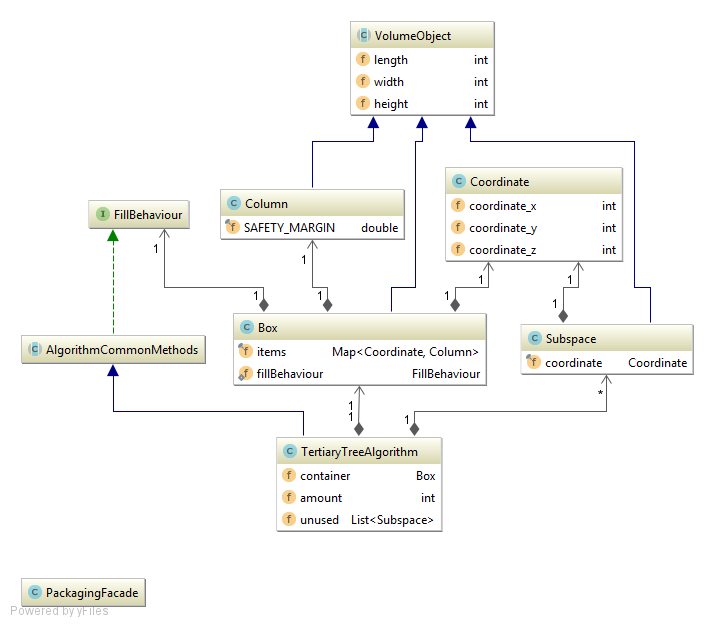
\includegraphics[width=17cm]{Class_diagram_packing_classes2.png}\\
In the packing algorithm, this is the first step that happens. The data entered in the front-end is passed through the rest-service, then the Facade, and finally arrives here. \\

A Strategy pattern is implemented for future algorithms. Right now, the Tertiary Tree Algorithm works only with 1 homogeneous object. In case you'd want to try a different algorithm or approach, you can just make a new class, implement FillBehaviour (or extend AlgorithmCommonMethods) and start coding. \\

The TertairyTreeAlgorithm will place Columns in subspaces, then divide that subspace in 3 other subspaces. This will keep going until the column no longer fits in the subspace. Whenever a column is placed, it will be mapped with a coordinate. \\

Keep in mind that the creation of objects is entirely done through factories.

\pagebreak


\subsection{Class diagram: Setup algorithm}
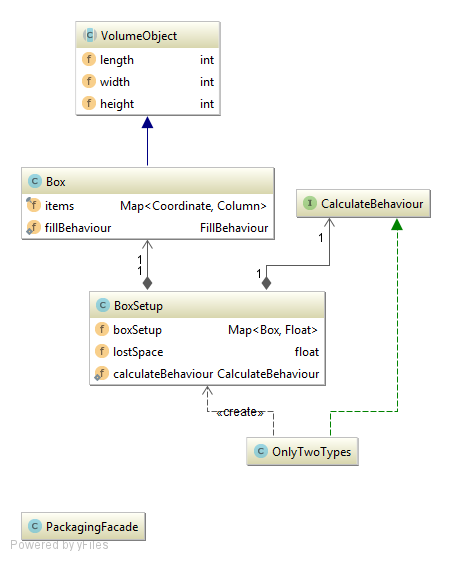
\includegraphics[width=12cm]{Class_diagram_setup_classes2.png}\\
These classes will determine what the best setup of boxes is. The packing algorithm will determine how much space is lost and how many columns can fit into a box. Afterwards, "BoxSetup" will determine (according to the previous data) how many boxes will be necessary.\\

This algorithm is not the most performant, as it brute-forces all possibilities and then chooses the one setup with the least volume loss.\\

\paragraph{There are 2 major drawbacks:}
\begin{enumerate}
	\item It is a brute force algorithm.
	\item Only 2 containers are supported in the "OnlyTwoTypes" class. A better algorithm can easily be implemented by making a new class, and implementing "CalculateBehaviour". 
\end{enumerate}

After choosing the best "BoxSetup", you'll return this to the Facade. Before returning it to the rest-service, it will be converted in another format. "TranslatorContainersetup" does this for you. After translating, it is sent to the rest-service. There it will be converted into JSON format.

\section{Maven configurations}
\subsection{back-end}
Please do remember that whenever you build this for the very first time, you must first "build \& install" it with maven so it is in your local repository. This is easily done with an IDE that supports maven Projects. \\

I'd like to focus on 2 parts of the "pom.xml" of the back-end project: 
\lstset{language=xml}
\begin{lstlisting}
	<groupId>com.bin</groupId>
	<artifactId>3dbinpackaging</artifactId>
	<version>1.4</version>
	
	<dependencies>
		<!-- https://mvnrepository.com/artifact/junit/junit -->
		<dependency>
			<groupId>junit</groupId>
			<artifactId>junit</artifactId>
			<version>4.12</version>
		</dependency>
	</dependencies>
\end{lstlisting}

The first part are the identification details about our back-end project. We'll need these later on when we import it in our rest-service. The second part is simply a JUnit dependency that you import.

\pagebreak
\subsection{rest-service}
\begin{lstlisting}
	<parent>
		<groupId>org.springframework.boot</groupId>
		<artifactId>spring-boot-starter-parent</artifactId>
		<version>1.5.2.RELEASE</version>
	</parent>
	
	<dependencies>
		<dependency>
			<groupId>com.bin</groupId>
			<artifactId>3dbinpackaging</artifactId>
			<version>1.4</version>
		</dependency>
		<dependency>
			<groupId>org.springframework.boot</groupId>
			<artifactId>spring-boot-starter-web</artifactId>
		</dependency>
		<dependency>
			<groupId>org.springframework.boot</groupId>
			<artifactId>spring-boot-starter-test</artifactId>
			<scope>test</scope>
		</dependency>
		<!-- https://mvnrepository.com/artifact/com.google.code.gson/gson -->
		<dependency>
			<groupId>com.google.code.gson</groupId>
			<artifactId>gson</artifactId>
			<version>2.8.0</version>
		</dependency>
	</dependencies>
\end{lstlisting}
Most of this is from the official \hyperref{https://spring.io/guides/gs/rest-service/}{}{}{spring rest service website}. This is to use Spring annotations, etc... \\

The other parts that are important, is first of all the dependency where you import the previously build project (the back-end). Make sure the versions match. \\

There is also the "gson" dependency. That's because we are mapping complex objects, and gson is (in my experience) easier to use. 

\pagebreak
\section{CORS and GSON complex serialization}
The default setting refuses JSON request that's not from the same origin. To disable this for specific routes, we have the following configuration in our "Application.java" file in the rest-service.

\lstset{language=Java}
\begin{lstlisting}
@SpringBootApplication
public class Application {
	public static void main(String[] args) {SpringApplication.run(Application.class,args);	}
		
		@Bean
		public WebMvcConfigurer corsConfigurer() {
			return new WebMvcConfigurerAdapter() {
				@Override
				public void addCorsMappings(CorsRegistry registry) {
					registry.addMapping("/api/**");
				}
		};
	}
}
\end{lstlisting}

Now all sorts of front-ends can send JSON requests to our application. \\

Because we work with complex objects (Maps in Maps, objects in objects), we'll have to configure GSON. This is done in your Controller class in the rest-service.
\begin{lstlisting}
@RestController
public class ContainerSetupController {
	GsonBuilder builder = new GsonBuilder().enableComplexMapKeySerialization().setPrettyPrinting();
	Gson gson = builder.create();
\end{lstlisting}

\pagebreak

\section{Nice implementations \& extensions }
This project is just meant as a stepping stone for a more automated and easier approach to calculate data. Of course, it does not stop there. With the second part, cost regression, programmed and implemented, a lot of steps can be automated. \\

\paragraph{Several ideas:}
\begin{itemize}
	\item Implement cost regression in the rest service, and adjust the front-end. \\
	this will encourage a complete, smooth, web-based approach. There are 3 advantages over Excel:
	\begin{enumerate}
		\item Right now (if I'm not mistaken) the Cost Regression that's made in Excel, uses Windows-only code and makes it OS dependent.
		\item Time is lost when copy-pasting data from the web application into the excel
		\item More futuristic opportunities, such as linking calculations to a database. Either to keep a history of orders, or for statistical analysis.
	\end{enumerate}
	\item Perhaps the generation of invoices?
	\item 3D visualization on the website / front-end
	\item Current boxes (dimensions) are an "Enum" file. This can either be kept in a configuration file, or database. \\ \\
\end{itemize}

Enum file as a reference:
\begin{lstlisting}
	public enum BoxType {
		SMALLEST(120,80,100),
		BIGGEST(150,100,120);
		
		private final int length;
		private final int width;
		private final int height;
		
		BoxType(int length, int width, int height) {
			this.length = length;
			this.width = width;
			this.height = height;
		}
\end{lstlisting}
\end{document}